\documentclass[11pt]{article}
\usepackage{geometry}
\geometry{margin=1in}
\usepackage{amsmath,amssymb}
\usepackage{booktabs}
\usepackage{graphicx}
\usepackage{hyperref}
\usepackage{siunitx}
\DeclareSIUnit\dimensionless{}  % define a “dimensionless” unit
\usepackage{float}
\usepackage{algorithm}
\usepackage{algpseudocode}   % from the algorithmicx package
\usepackage{tikz}
\usetikzlibrary{shapes.geometric, arrows.meta, positioning, fit}
\usepackage{caption}
\captionsetup{font=small,labelfont=bf}

\title{\bfseries AuctioNN: A Simulation-Driven Bidding Engine for\\
Large-Scale Cost-Per-Action Optimization}
\author{Param Kapur, Cameron Adams, Quinn Behrens, Ernie Zhang \\
\texttt{\{paramkapur, cadams, qbehrens, irenez\}@reed.edu}\\}
\date{\today}

\begin{document}
\maketitle
\vspace{-1em}

\begin{abstract}
  \noindent
  \textbf{AuctioNN} is a sandbox framework and decision engine that
  evaluates whether a \emph{neural-network–guided bidding policy} can
  reduce system-wide cost-per-action~(CPA) while meeting
  campaign-specific goals and operational constraints.  The
  instrumented simulator streams impression requests one at a time,
  emulating an external, first-price and second-price ad exchange.
  We rigorously
  compare the proposed policy against heuristic baselines using
  \emph{marginal CPA}, total conversions, and revenue uplift.
  Results generalize to media owners such as~\emph{iHeart} that
  simultaneously monetize their owned\&operated (O\&O) inventory and
  purchase incremental reach on open exchanges.  The full
  architecture, mathematical formulation, and open research questions
  are documented here. %
\end{abstract}

\section{Introduction}

Online advertising operates at a staggering scale, with billions of individual auctions happening every day across the web, apps, and streaming platforms. At the core of this system lies the real-time bidding (RTB) process, where advertisers compete to show their ads to specific users at specific moments. But not all impressions are created equal, some users are far more likely to engage, click, or convert than others. The challenge, then, is to bid intelligently: to spend money where it is most likely to drive meaningful outcomes, such as purchases, signups, or app installs, while respecting the constraints of campaign budgets and performance goals.

Large media publishers increasingly extend their reach by \emph{buying} impressions on open ad exchanges. Operating \num{e3}--\num{e4} concurrent campaigns in real time raises three entangled challenges:
\begin{enumerate}
  \item \textbf{Win the \emph{right} inventory}—impressions that
    drive post-click or post-view conversions.
  \item \textbf{Respect campaign goals}—especially CPA targets
    stipulated in insertion orders.
  \item \textbf{Obey operational constraints}—budgets, pacing, and
    user-level frequency capping.
\end{enumerate}
This work posits that a neural model, combined with explicit budget/frequency bookkeeping, can outperform classical heuristics that ignore conversion likelihood, or at the very least, random bidding.

Traditionally, bidding strategies in RTB have either relied on simple heuristics, such as bidding proportionally to an advertiser's declared value per conversion, or leveraged machine learning models that directly output a recommended bid price based on the enviroment. Much of the recent work in this space has focused on reinforcement learning (RL) approaches, where an agent learns a bidding policy through interaction with an environment, balancing exploration with campaign-level constraints like budget or cost-per-action (CPA) targets.

Our approach takes a different path. Rather than asking the neural network to output a bid price directly, we use it to focus on \emph{what we believe to be the root of the problem}: predicting the likelihood that a given impression will result in a conversion. In other words, we train a neural network purely as a \emph{conversion predictor}, separate from the bidding logic itself. We then use this predicted probability as an input to a decision (auction) algorithm that determines whether to bid, on which campaign, and at what price.

The key motivation for this work is that accurate conversion estimation can enable more principled and interpretable bidding decisions. This separation of concerns allows the model to specialize in what it does best (learning conversion patterns from data) while keeping the bidding policy flexible and transparent.

In this paper, we present \emph{AuctioNN}, a simulation driven bidding engine that integrates neural network based conversion prediction into the bidding process. We compare our system against heuristic baselines and explore whether this two-stage approach can outperform strategies that directly optimize the bid price. Along the way, we hope to clarify how learning better \emph{conversion likelihoods}, rather than directly learning \emph{bids}, can lead to simpler, scalable, and more interpretable auction strategies.


\section{Background}

\subsection{The Landscape of Bidding in Online Advertising}

At the heart of real-time bidding (RTB) systems is a deceptively simple question: \emph{how much should an advertiser bid for a given ad impression?} Yet behind this question lie several layers of complexity. The auction mechanisms themselves may vary (first-price, second-price, programmatic guaranteed), campaign objectives often include a mix of budget limits and cost-per-action (CPA) goals, and, critically, the true value of an impression (whether it will lead to a conversion) is rarely known at the time of bidding.

Historically, the first generation of bidding strategies relied on \emph{rule-based heuristics}. These approaches often computed the expected value of an impression by estimating the probability of a click (CTR) or conversion (CVR) and then multiplying this probability by the advertiser’s declared value per click or per conversion. The bid was then set either directly to this expected value or scaled by a constant factor to account for risk preferences or auction mechanics. These heuristics worked well in the early days of second-price auctions, where truthful bidding (bidding your true value) is an optimal strategy under ideal conditions.

However, with the majority of online auctions being  \emph{first-price auctions}, where the winning bidder pays their own bid amount, disrupted this simplicity. In first-price environments, bidding your full value results in systematically overpaying, so bidders must ``shade'' their bids downward to avoid eroding profit margins. This need for bid shading introduced a new layer of strategic uncertainty, where bidders had to model not just their own value but also anticipate the distribution of competing bids.

\subsection{How an Open Ad Exchange Works}
\label{sec:exchange}

For each page-view or app launch, the exchange issues a \emph{bid
request} containing contextual metadata (timestamp, device, geo,
etc.).  Every buyer has roughly \SI{100}{\milli\second} to (i) decide
whether to participate and (ii) transmit a bid price.
The highest bid wins and immediately pays the \emph{clearing price}.
In most modern exchanges this is a \emph{first-price auction}; the
winner pays its own bid. However, some exchanges use different auction
models like \emph{second-price} or programmatic guaranteed (PG) auctions.
Any downstream \emph{conversion event} (purchase, signup, \dots) is
reported asynchronously, often minutes to days later.

\subsection{Reinforcement Learning for Bidding: Direct Bid Optimization}

As these complexities grew, researchers began turning to \emph{reinforcement learning (RL)} to optimize bidding strategies. In this framework, bidding is modeled as a sequential decision-making problem, where the agent interacts repeatedly with an environment (the auction marketplace), and learns a policy that maximizes long-term rewards (e.g., total conversions, clicks, or revenue) while respecting budgetary or pacing constraints.

One early influential approach was the \emph{Real-Time Bidding by Reinforcement Learning (RLB)} framework by Cai et al.\ (2017). This work framed bidding as a Markov Decision Process (MDP), where the state included remaining budget, remaining time, and other campaign features. The action space was the set of possible bid prices. The RLB agent used value-based RL methods to learn the expected cumulative reward from each state-action pair and selected bids accordingly. The reward function was typically tied to immediate outcomes like clicks or conversions.

Following this, Wu et al.\ (2018) addressed an important limitation of the basic RLB approach: naïve reward structures can lead to poor budget pacing, with agents spending too aggressively early in a campaign or failing to adapt to delayed conversion feedback. To remedy this, Wu et al.\ introduced \emph{budget-aware state representations} and carefully designed reward functions that penalized over- or under-spending relative to pacing goals. Their approach allowed the RL agent to account for the long-term impact of current bidding decisions on campaign success, making it more robust in practice.

Further advancements leveraged \emph{actor-critic methods} and \emph{policy gradient techniques}, which provided greater flexibility in handling continuous bid values and more stable learning dynamics. For example, Liu et al.\ (2021) introduced a \emph{Soft Actor-Critic (SAC)} approach to bidding, which incorporated entropy regularization to encourage exploration and avoid premature convergence to suboptimal bidding strategies. Instead of outputting a hard bid price directly, their system learned a distribution over bid adjustment factors, allowing for more nuanced bidding behavior under uncertainty.

In many of these RL-based systems, the \emph{neural network learns the bidding policy itself}, meaning that the network outputs the bid amount or bid adjustment as a function of the input state. Conversion probabilities may still be implicitly learned within the network, but they are not exposed directly as outputs or decision-making inputs. Instead, the network collapses prediction and decision-making into a single policy.

\subsection{Conversion Prediction as a Separate Task}

A parallel thread of research in online advertising focuses on \emph{conversion rate prediction (CVR)} and \emph{click-through rate prediction (CTR)} as standalone supervised learning tasks. These models, often logistic regression or gradient-boosted trees, take impression features (user metadata, time of day, device type, etc.) and predict the likelihood that a given impression will lead to a conversion.

The outputs of these models are typically used as \emph{inputs into heuristic bidding rules}. A common strategy is to bid proportionally to the predicted conversion probability times the advertiser's declared value per conversion. For example, if the CVR is 1\% and the conversion is worth \$100, the bid might be \$1 (or shaded downward in a first-price setting).

Google's \emph{Smart Bidding} strategies, as well as Facebook’s auction system, are examples of large-scale production systems where machine learning predicts the likelihood of various outcomes and then uses those predictions to guide bidding decisions. However, in many of these systems, the predictive model itself is \emph{deeply coupled} with the bidding logic, and the specifics of how conversion probabilities are used within the bid calculation are proprietary. This is the path our model will utalize.

\subsection{The Gap: Prediction vs.\ Policy}

The central observation motivating our work is that \emph{most reinforcement learning and direct policy-learning approaches collapse prediction and bidding into a single learned function}, whereas supervised conversion prediction models are typically used only within simple heuristic bidding formulas.

We believe there is value in keeping these two steps distinct.

Our work builds on the idea that \emph{accurate prediction of conversion likelihood is a critical first step}, and that bidding should then be handled by a separate, explicitly defined decision engine. This separation has several advantages:

\begin{itemize}
    \item \textbf{Interpretability}: The predicted conversion probability is a meaningful, transparent quantity that can be audited, analyzed, and improved independently of the bidding logic.
    \item \textbf{Flexibility}: The bidding strategy can be easily adjusted (e.g., to change the aggressiveness of bid shading or apply new campaign constraints) without retraining the prediction model.
    \item \textbf{Modularity}: Improvements in the conversion predictor (e.g., better features, better model architecture) directly enhance the quality of the inputs to the bidding engine, without requiring changes to the decision logic.
\end{itemize}

\subsection{How Our Approach Fits In}

In this paper, we propose \emph{AuctioNN}, a bidding engine that explicitly separates \emph{conversion prediction} from \emph{bid decision-making}. AuctioNN uses a neural network to estimate the probability of conversion for each impression-campaign pair. This probability feeds into a bid selection rule that incorporates campaign-specific parameters such as target CPA, budget pacing, and frequency capping.

This approach is influenced by several lines of past research:

\begin{itemize}
    \item From \textbf{heuristic bidding models}, we inherit the principle that bids should reflect expected value (predicted conversion probability times value per conversion).
    \item From \textbf{supervised learning approaches to CVR modeling}, we adopt the use of predictive models trained on historical data to estimate conversion likelihoods.
    \item From \textbf{reinforcement learning and auction theory}, we recognize the importance of long-term planning, pacing, and strategy under first-price auction dynamics.
\end{itemize}

However, we intentionally \emph{do not use the neural network to directly output bids}, nor do we collapse the policy into the model itself. Instead, we leverage the predictive model as an informed signal within a broader bidding framework. This distinction allows us to maintain interpretability, modularity, and flexibility while still benefiting from the power of neural networks for learning complex patterns in the data.

\section{System Architecture \& Environment}\label{sec:env}

AuctioNN treats the exchange as an online stream, delivering
impression~$I_t$ at discrete time~$t$.
For every impression the engine must
\emph{(a)} decide whether to bid,
\emph{(b)} pick a campaign, and
\emph{(c)} set the bid price.
Table~\ref{tab:variables} formalizes the symbols used throughout the paper.

\begin{table}[H]
  \centering
  \caption{Core symbols and state variables.}
  \label{tab:variables}
  \begin{tabular}{ll}
    \hline
    Symbol / Term & Meaning \\
    \hline \\
    $I_t$ & Impression delivered at discrete time~$t$. \\
    $\mathrm{features}(I_t)$ & All metadata included in the bid request. \\
    $C$ & Active campaign set. \\
    $c \in C$ & One specific campaign. \\
    $\mathrm{budget\_remaining}[c]$ & Dollars left for campaign~$c$. \\
    $p_{\mathrm{conv}}(c,I_t)$ & Predicted conversion probability
    if~$c$ wins~$I_t$. \\
    $\mathrm{value\_per\_conv}[c]$ & Advertiser-declared value of one
    conversion. \\
    $\mathrm{target\_CPA}[c]$ & Optional maximum CPA for campaign~$c$. \\
    $\mathrm{ad\_stock}[\text{user},c]$ & Recent exposure score
    (models ad fatigue). \\
    $\mathrm{score}(c,I_t)$ & Scalar used to select the winning campaign. \\
    $\mathrm{bid}$ & Dollar price sent to the exchange. \\
    $\mathrm{clearing\_price}$ & Amount paid if the bid wins
    ($=\mathrm{bid}$ in first-price). \\
    $\mathrm{marginal\;CPA}$ & $\Delta\text{Spend} /
    \Delta\text{Conversions}$ over a window.\\
  \end{tabular}
\end{table}

% ------------------------------------------------------------
\subsection{End-to-End Decision Loop}\label{sec:decisionloop}
The procedure below executes for \emph{every} incoming impression.

\begin{algorithm}[H]
  \caption{AuctioNN per-impression decision loop}
  \begin{algorithmic}[1]
    \Require incoming impression $I_t$
    \State \textbf{Receive} $I_t$; extract $\mathrm{features}(I_t)$
    \State \textbf{Eligibility gate}:\\
    \hspace{\algorithmicindent}%
    $C_{\text{elig}}\!\gets\!\{c\!\in\!C\mid
      \texttt{budget\_remaining}[c]>0\ \land\
    \texttt{ad\_stock}[\text{user},c]<\tau\}$
    \ForAll{$c\in C_{\text{elig}}$}
    \State $p_{\mathrm{conv}}(c,I_t)\gets
    f_{\theta}\bigl(\mathrm{features}(I_t),
      \mathrm{embed}(c),
    \mathrm{ad\_stock}[\text{user},c]\bigr)$ \hfill$\triangleright$
    see §\ref{sec:nn}
    \State $\mathrm{score}(c,I_t)\gets
    \begin{cases}
      \displaystyle\frac{p_{\mathrm{conv}}}{\mathrm{target\_CPA}[c]}, &
      \text{if target\_CPA exists},\\
      p_{\mathrm{conv}}\times\mathrm{value\_per\_conv}[c], &
      \text{otherwise.}
    \end{cases}$
    \EndFor
    \State $c^{\ast}\gets\arg\max_{c}\mathrm{score}(c,I_t)$
    \State $\mathrm{expected\_value}\gets
    p_{\mathrm{conv}}(c^{\ast},I_t)\times
    \mathrm{value\_per\_conv}[c^{\ast]}$
    \State $\mathrm{bid}\gets\beta\times\mathrm{expected\_value}$
    \Comment{$\beta=1$ initially\footnotemark}
    \State \textbf{Transmit} $\mathrm{bid}$; observe win/loss and
    $\mathrm{clearing\_price}$
    \If{win}
    \State $\texttt{budget\_remaining}[c^{\ast}] \mathrel{-}=
    \mathrm{clearing\_price}$
    \State $\mathrm{ad\_stock}[\text{user},c^{\ast}] \mathrel{+}= 1$
    \EndIf
    \State Log \textit{(}$I_t$, $c^{\ast}$, bid, win/loss, time,
    utility\textit{)} for offline analysis
  \end{algorithmic}
  \footnotetext{We begin with a trivial “no shading’’ policy
    ($\beta=1$); developing a risk-adjusted shading strategy is left
  for future work.}
\end{algorithm}
% ------------------------------------------------------------

\subsection{Decision Loop Pipeline}\label{sec:decisionloop}
The figure below illustrates the decision loop in a block diagram.

% ---------------------------------------------------------------
%  AuctioNN: cleaned block diagram with compound Inference+Select
% ---------------------------------------------------------------
\begin{figure}[H]
  \centering
  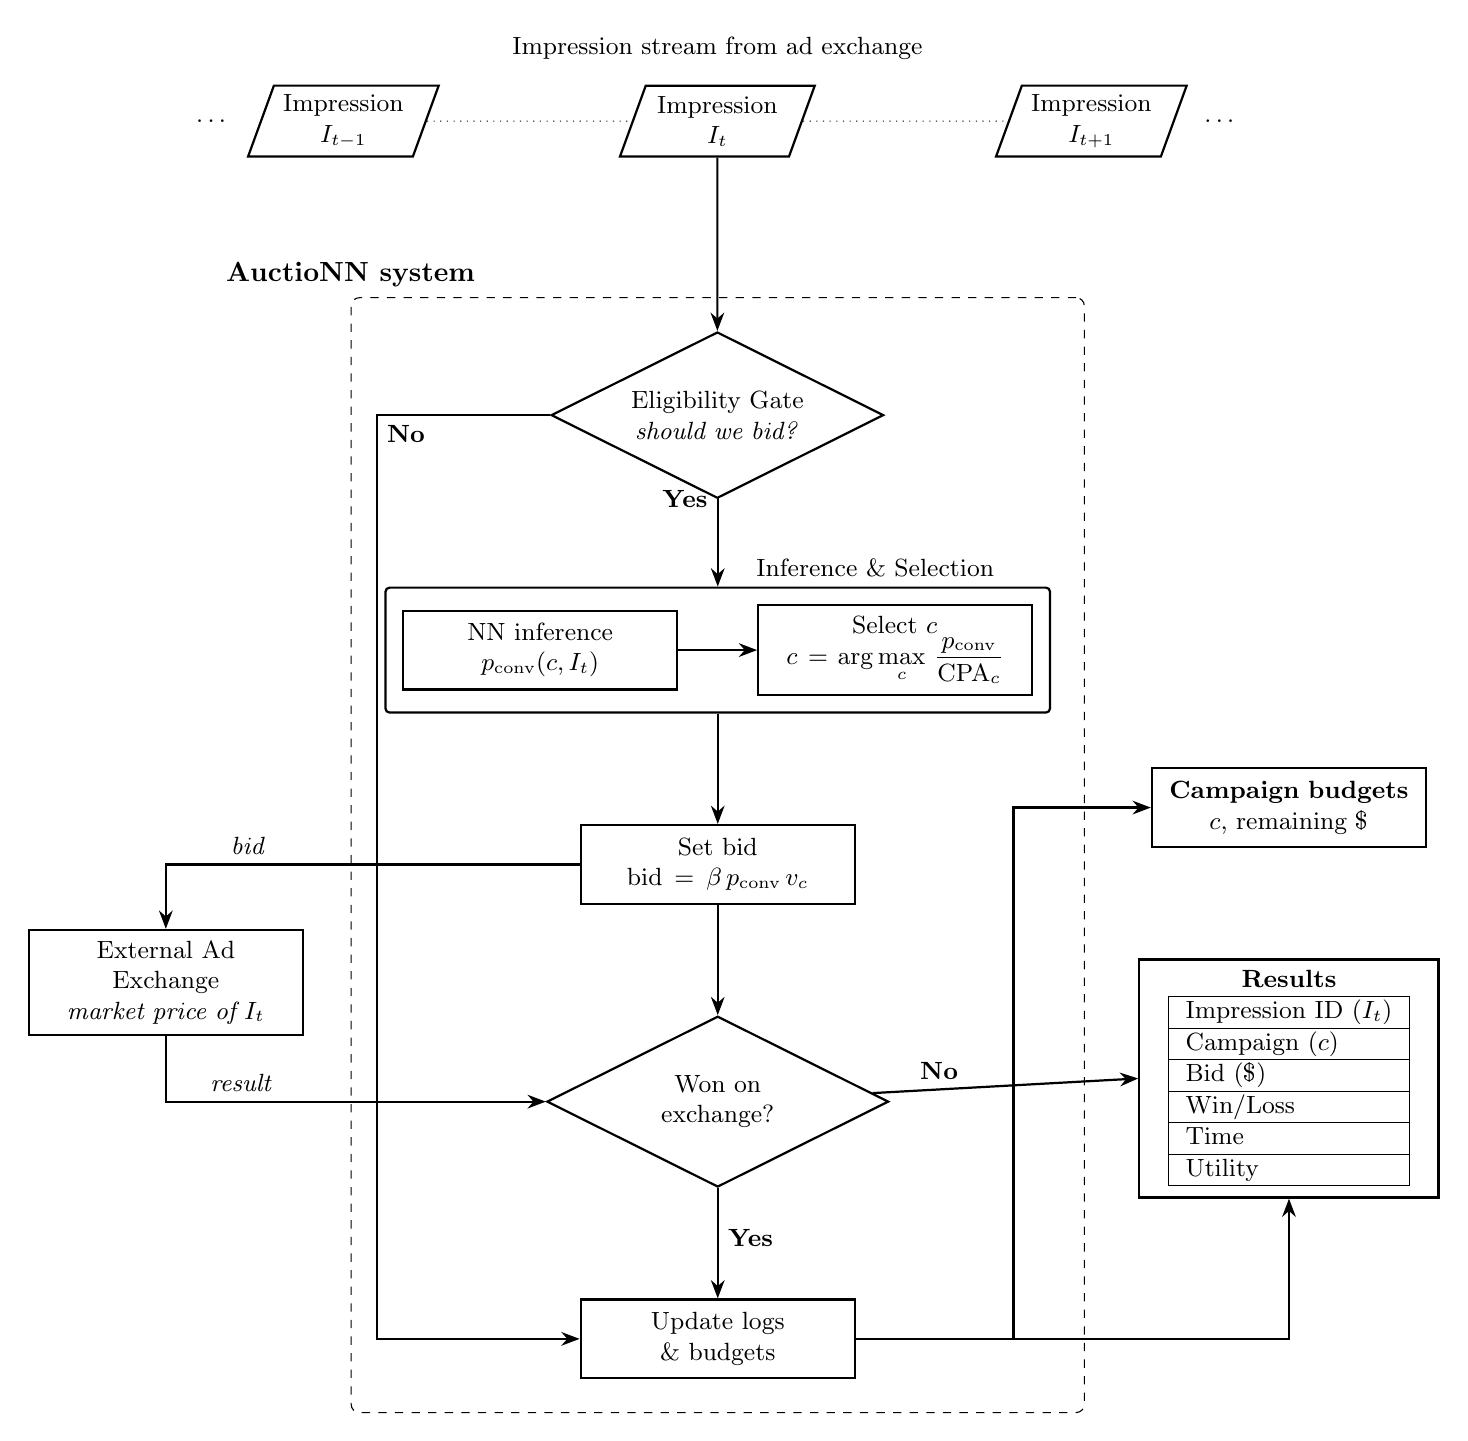
\begin{tikzpicture}[
      font=\small,
      node distance = 14mm and 26mm,
      >=Stealth,
      line/.style      = {thick,->},
      block/.style     = {rectangle, draw, thick, align=center,
        text width=32mm, inner sep=4pt,
      minimum height=10mm},
      decision/.style  = {diamond, draw, thick, align=center,
      aspect=2, inner sep=1pt, text width=28mm},
      io/.style        = {trapezium, draw, thick, align=center,
        trapezium left angle=70, trapezium right angle=110,
      minimum width=22mm, minimum height=9mm},
      dashedBox/.style = {draw, dashed, rounded corners=3pt, inner sep=12pt},
      compoundBox/.style = {rectangle, draw, thick, rounded corners=1.5pt,
      inner sep=6pt}
    ]

    % ---------------- impression stream ----------------
    \node[io]                       (impPrev) {Impression\\$I_{t-1}$};
    \node[io, right=of impPrev]     (imp)     {Impression\\$I_t$};
    \node[io, right=of imp]         (impNext) {Impression\\$I_{t+1}$};

    \node[above=2mm of imp, font=\small] (streamLabel)
    {Impression stream from ad exchange};

    \draw[dotted] (impPrev) -- (imp) -- (impNext);
    \node[right=0.25cm of impNext] (dotsR) {$\dots$};
    \node[left=0.25cm of impPrev]  (dotsL) {$\dots$};

    % ---------------- decision loop ----------------
    \node[decision, below=22mm of imp]  (gate)
    {Eligibility Gate\\\textit{should we bid?}};

    % --- compound Inference + Selection block ---
    % sub-blocks
    \node[block, below=of gate, xshift=-2.25cm]         (nn)
    {NN inference\\$p_{\text{conv}}(c,I_t)$};
    \node[block, right=10mm of nn]      (argmax)
    {Select $c^{\*}$\\$\displaystyle
    c^{\*}=\arg\max_{c}\,\frac{p_{\text{conv}}}{\text{CPA}_c}$};
    % enclosing box
    \node[compoundBox, fit=(nn)(argmax), label=north:{ \hspace{4cm}Inference
    \& Selection}]
    (infsel) {};

    % remaining blocks
    \node[block, below=of infsel] (bid)
    {Set bid\\$\text{bid}=\beta\,p_{\text{conv}}\,v_c$};
    \node[decision, below=of bid] (win?)
    {Won on\\exchange?};
    \node[block, below=of win?]   (update)
    {Update logs\\\& budgets};

    % dashed container around whole logic
    \node[dashedBox, fit=(gate)(infsel)(bid)(win?)(update)] (sysbox){};
    \node[above=0pt of sysbox.north west, font=\bfseries] {AuctioNN system};

    % ---------------- external tables ----------------
    \node[block, right=60mm of nn, yshift=-2cm] (budget)
    {\textbf{Campaign budgets}\\$c$, remaining \$};
    \node[block, below=of budget, minimum width=38mm,
    minimum height=23mm] (results) {
      \textbf{Results}\\[2pt]
      \begin{tabular}{|l|}
        \hline Impression ID ($I_t$)\\ \hline
        Campaign ($c$)\\ \hline
        Bid (\$)\\ \hline
        Win/Loss\\ \hline
        Time\\ \hline
        Utility\\ \hline
    \end{tabular}};

    \node[block, left=35mm of bid, yshift=-15mm] (exchange)
    {External Ad Exchange\\\textit{market price of $I_t$}};

    % ---------------- arrows (main flow) -------------
    \draw[line] (imp) -- (gate.north);

    \draw[line] (gate.south) -| node[left]{\bfseries
    Yes} (infsel.north);
    \draw[line] (nn) -- (argmax);
    \draw[line] (infsel.south) -- (bid.north);

    \draw[line] (bid.south) -- (win?.north);

    \draw[line] (win?.south) -- node[right, yshift=2pt]{\bfseries Yes} (update);

    % ---------------- arrows (side paths) ------------
    % No-bid branch
    \draw[line] (gate.west) -- ++(-22mm,0) |- node[right,
    pos=0.01]{\bfseries No}
    (update.west);

    % bid to exchange
    \draw[line] (bid.west) -| node[above, pos=0.4]{\textit{bid}}
    (exchange.north);
    % result back
    \draw[line] (exchange.south) |- node[above, pos=0.6]{\textit{result}}
    (win?.west);

    % win? -> results  (No branch)
    \draw[line] (win?) -- node[near start, above]{\bfseries No}
    (results.west);

    % update -> budgets & results
    \draw[line] (update.east) -- ++(20mm,0) |- (budget.west);
    \draw[line] (update.east) -- ++(10mm,0) -| (results.south);

  \end{tikzpicture}
  \caption{Fully connected block diagram of AuctioNN’s
    \emph{per-impression} decision loop, emphasising the continuous stream
    of impressions \(I_{t-1}, I_t, I_{t+1}, \dots\).  The compound
    \emph{Inference \& Selection} stage first scores every campaign with a
    neural network and then chooses \(c^{\*}\) via the displayed arg-max
  rule.}
  \label{fig:auctionn-loop-final}
\end{figure}
\newpage

\vspace{-0.5em}
% --------------------------------------------------------------------
\section{Neural Model}\label{sec:nn}
% --------------------------------------------------------------------

\subsection{Feature Representation}

We structure the impression data into two categories of features:

\begin{itemize}
  \item \textbf{Categorical features (10 total):} Each categorical feature is first integer-encoded and then mapped into a \SI{32}{\dimensionless}-dimensional embedding vector. These include ad-placement details (e.g., placement ID, DMA, country), user-agent characteristics (e.g., browser, OS, device family), and crucially, the campaign identifier itself.
  
  \item \textbf{Numerical features (8 total):} We incorporate boolean flags indicating device attributes (e.g., mobile or tablet usage) and encode temporal signals—such as hour-of-day and day-of-week—using cyclical sine/cosine transformations. Each numerical feature is standardized via z-score normalization.
\end{itemize}

\subsection{Network Architecture}

The neural network itself is a compact Multi-Layer Perceptron (MLP) designed to predict the probability of conversion conditioned jointly on impression features and campaign identity. Specifically, the campaign ID is treated as just another categorical input, allowing the model to naturally learn campaign-specific conversion tendencies. During inference, we can easily swap in any campaign ID to predict how that campaign would perform for a given impression.

The network processes input as follows:

\[
\begin{aligned}
\mathbf{e} &= \bigoplus_{f\in\mathcal{C}} \operatorname{Embed}_{f}(x_{f}) &&\in\mathbb{R}^{10\times32}\\
\mathbf{z} &= [\,\mathbf{e}\;\|\;\mathbf{x}_{\text{num}}\,] &&\in\mathbb{R}^{328}\\
\mathbf{h}_1 &= \operatorname{ReLU}\bigl(\operatorname{BN}_{1}(\mathbf{W}_1\mathbf{z} + \mathbf{b}_1)\bigr)\\
\mathbf{h}_2 &= \operatorname{ReLU}\bigl(\operatorname{BN}_{2}(\mathbf{W}_2\mathbf{h}_1 + \mathbf{b}_2)\bigr)\\
\ell &= \mathbf{w}_{\text{out}}^{\top}\mathbf{h}_2 + b_{\text{out}}\\[2pt]
p_{\text{conv}} &= \sigma(\ell)
\end{aligned}
\]

The model comprises two hidden layers with 128 and 64 neurons, each followed by batch normalization and a dropout rate of 0.3, totaling roughly 55,000 parameters. It is trained using the Adam optimizer with a learning rate of \(10^{-3}\) and a batch size of 2048 over 10 epochs. To handle the severe class imbalance in the data, we employ weighted binary cross-entropy loss (\(\text{pos\_weight} = 137.0\)).

\subsection{Current Performance}

Table~\ref{tab:metrics} summarizes the validation results obtained after training on a dataset of approximately 3.85 million impressions (15\% validation split). \textbf{Please note that this dataset comprised of only ONE campaign. We are yet to train on all 100 campaigns.}

\begin{table}[H]
  \centering
  \caption{Validation metrics after 10 epochs of training}
  \label{tab:metrics}
  \begin{tabular}{l@{\quad}S}
    \toprule
    Metric & {Value} \\
    \midrule
    ROC–AUC & 0.9295 \\
    PR–AUC (average precision) & 0.4347 \\
    Log loss & 0.2849 \\
    Accuracy @{0.5} & 0.8896 \\
    Precision @{0.5} & 0.0493 \\
    Recall @{0.5} & 0.7791 \\
    F$_1$ @{0.5} & 0.0928 \\
    \midrule
    True negatives (TN) & \num{509935} \\
    False positives (FP) & \num{62756}  \\
    False negatives (FN) & \num{923}      \\
    True positives (TP) & \num{3256}   \\
    \bottomrule
  \end{tabular}
\end{table}

The model achieves excellent predictive quality (ROC–AUC \(>\)0.92), although precision remains challenging due to the high class imbalance inherent in conversion data.

\subsection{Future Improvements}

To further enhance the model's capability, we plan several improvements:

\begin{itemize}
  \item Introduce a balanced data sampling strategy during training to ensure the model learns effectively across campaigns of varying sizes.
  \item Optimize inference by vectorizing model predictions, allowing scoring of all 100 candidate campaigns simultaneously instead of individually.
  \item Enhance training stability through adaptive learning rate schedules (ReduceLROnPlateau), early stopping criteria, and experimenting with focal loss to better handle extreme class imbalances.
  \item Regularize campaign embeddings (via L2 penalties) and introduce techniques such as negative sampling or data augmentation to improve generalization on sparse or unseen campaign-impression combinations.
\end{itemize}



\section{Evaluation Methodology}\label{sec:evaluation}
We benchmark three policies: [WORK IN PROGRESS]

\begin{enumerate}
  \item \textbf{Random}—bid a constant \$1 CPM on a random eligible campaign.
  \item \textbf{Heuristic}—industry default: bid proportional to
    campaign value, ignoring $p_{\mathrm{conv}}$.
  \item \textbf{AuctioNN (proposed)}—full decision loop of
    §\ref{sec:decisionloop}.
\end{enumerate}

\subsection{Success Metrics}
\begin{itemize}
  \item \textbf{Marginal CPA}
    (\(\Delta\)Spend\(/\)\(\Delta\)Conversions) relative to baseline.
  \item \textbf{Total conversions} aggregated across all campaigns.
  \item \textbf{Revenue uplift} (= advertiser value – media cost).
  \item \textbf{Pacing error}:
    $|\mathrm{actual\;spend}-\mathrm{planned\;spend}|/\mathrm{planned\;spend}\le0.05$.
  \item \textbf{Latency}: distributive
    $p_{95}\le\SI{2}{\milli\second}$ per impression on a MacBook
    M-series laptop.
\end{itemize}

%--------------------------------------------------------------------
\section{Implementation Notes}\label{sec:implementation}
%--------------------------------------------------------------------

\subsection{Repository Layout}

\begin{verbatim}
auctionn_sim/
  - campaign.py            % Campaign dataclass + bootstrapper
  - exchange.py            % ImpressionGenerator, OnlinePreprocessor, Market
  - decision_loop.py     % Algorithm 1 implementation
  - logger.py            % Parquet-backed ResultsLogger
  - models/                % best_model.pth  (TorchScript or state-dict)
  - preprocessors/         % encoder / scaler artefacts
  - main.py                % CLI entry point
\end{verbatim}

\subsection{Impression Stream}
[WORK IN PROGRESS]
The gist of the implementation is as follows:
\begin{itemize}
  \item We generate a stream of Impression objects, from the data file using the ImpressionGenerator.
  \item We preprocess each Impression object using the OnlinePreprocessor so that we can use it for model inference.
  \item We pass each Impression object to the DecisionLoop, which returns a bid, win/loss, and clearing price.
  \item We update the ResultsLogger with the results.
\end{itemize}

\subsection{CLI Driver}

\begin{verbatim}
python run_sim.py \
    --data data/clean_data.parquet \
    --model models/best_model.pth \
    --preproc preprocessors/ \
    --out runs/run_01.parquet \
    --num-imps 1_000_000 \
    --device auto
\end{verbatim}


\section{Open Questions and Future Work}\label{sec:openq}

\section{Conclusion}
AuctioNN provides a controlled environment to test whether modern ML
can simultaneously optimise CPA, satisfy campaign obligations, and
execute within the harsh latency limits of real-time bidding.  The
architecture is intentionally minimal yet extensible, enabling
rigorous \emph{ablation studies} of every engineering choice—from
eligibility gates to neural features to bid shading policies.

% ----------------------------------------------------------------------
\bibliographystyle{plain}
\bibliography{auctionn}
\end{document}
